% arara: pdflatex

\documentclass[12pt,a4paper, landscape]{article}
\usepackage{tikz}
\usetikzlibrary{shapes,positioning,calc}
\colorlet{lightgray}{gray!20}

\usepackage{geometry}
 \geometry{
 a4paper,
 right=15mm,
 left=15mm,
 top=15mm,
 bottom=15mm
 }

\begin{document}

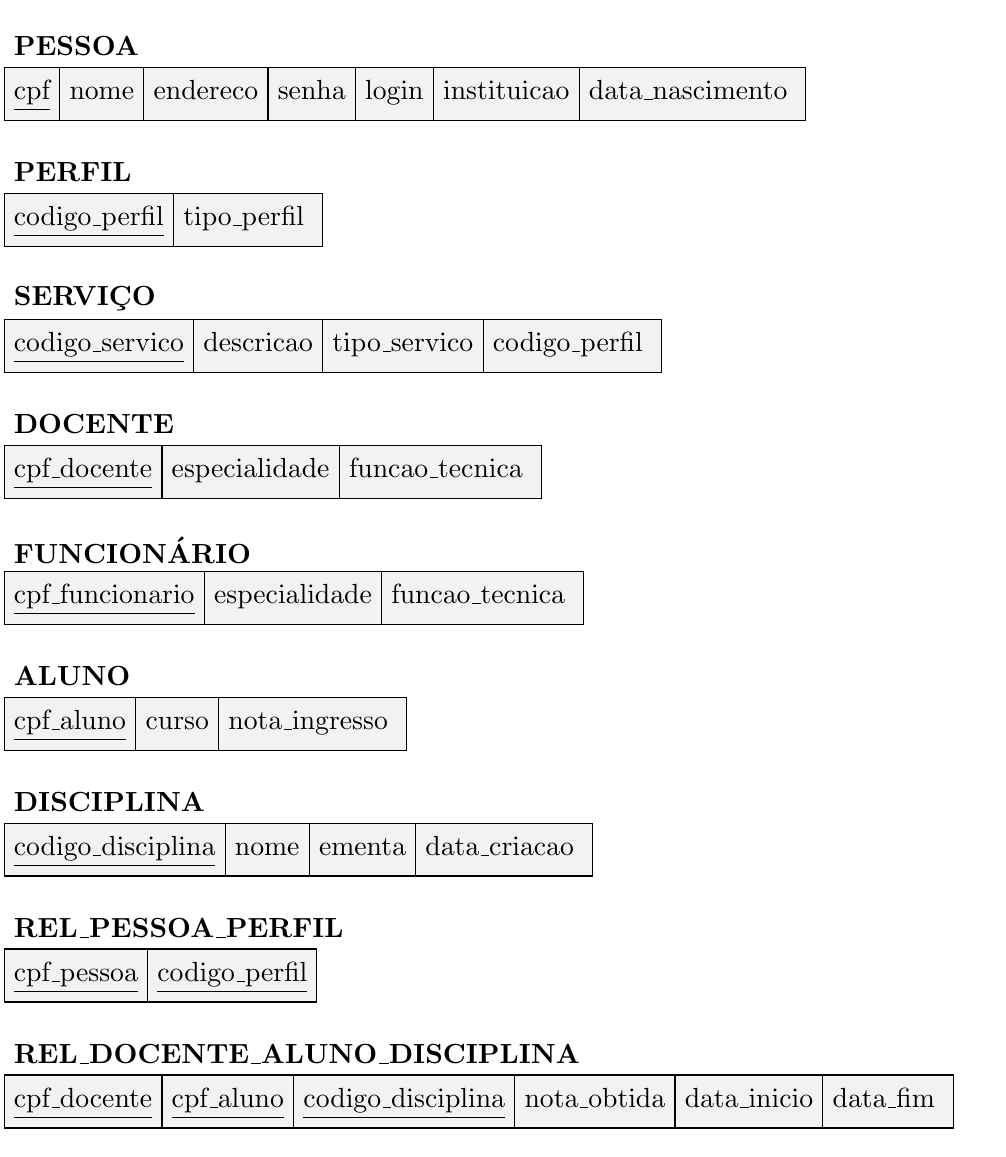
\begin{tikzpicture}[relation/.style={rectangle split, rectangle split parts=#1, rectangle split part align=base, draw, anchor=center, align=center, text height=3mm, text centered}]\hspace*{-0.3cm}

% RELATIONS

\node (pessoa-titulo) {\textbf{PESSOA}};

\node [relation=7, rectangle split horizontal, rectangle split part fill={lightgray!50}, anchor=north west, below=0.6cm of pessoa-titulo.west, anchor=west] (pessoa)
{\underline{cpf}%
\nodepart{two}   nome
\nodepart{three} endereco
\nodepart{four} senha
\nodepart{five} login
\nodepart{six} instituicao
\nodepart{seven} data\_nascimento
};

\node [below=1cm of pessoa.west, anchor=west] (perfil-titulo) {\textbf{PERFIL}};

\node [relation=2, rectangle split horizontal, rectangle split part fill={lightgray!50}, below=0.6cm of perfil-titulo.west, anchor=west] (perfil)
{\underline{codigo\_perfil}%
\nodepart{two} tipo\_perfil
};

\node [below=1cm of perfil.west, anchor=west] (servico-titulo) {\textbf{SERVIÇO}};

\node [relation=4, rectangle split horizontal, rectangle split part fill={lightgray!50}, anchor=north west, below=0.6cm of servico-titulo.west, anchor=west] (servico)
{\underline{codigo\_servico}%
\nodepart{two}   descricao
\nodepart{three} tipo\_servico
\nodepart{four} codigo\_perfil
};

\node [below=1cm of servico.west, anchor=west] (docente-titulo) {\textbf{DOCENTE}};

\node [relation=3, rectangle split horizontal, rectangle split part fill={lightgray!50}, anchor=north west, below=0.6cm of docente-titulo.west, anchor=west] (docente)
{\underline{cpf\_docente}%
\nodepart{two}   especialidade
\nodepart{three} funcao\_tecnica
};

\node [below=1cm of docente.west, anchor=west] (funcionario-titulo) {\textbf{FUNCIONÁRIO}};

\node [relation=3, rectangle split horizontal, rectangle split part fill={lightgray!50}, anchor=north west, below=0.6cm of funcionario-titulo.west, anchor=west] (funcionario)
{\underline{cpf\_funcionario}%
\nodepart{two}   especialidade
\nodepart{three} funcao\_tecnica
};

\node [below=1cm of funcionario.west, anchor=west] (aluno-titulo) {\textbf{ALUNO}};

\node [relation=3, rectangle split horizontal, rectangle split part fill={lightgray!50}, anchor=north west, below=0.6cm of aluno-titulo.west, anchor=west] (aluno)
{\underline{cpf\_aluno}%
\nodepart{two}   curso
\nodepart{three} nota\_ingresso
};

\node [below=1cm of aluno.west, anchor=west] (disciplina-titulo) {\textbf{DISCIPLINA}};

\node [relation=4, rectangle split horizontal, rectangle split part fill={lightgray!50}, anchor=north west, below=0.6cm of disciplina-titulo.west, anchor=west] (disciplina)
{\underline{codigo\_disciplina}%
\nodepart{two}   nome
\nodepart{three} ementa
\nodepart{four} data\_criacao
};

\node [below=1cm of disciplina.west, anchor=west] (relacao-pessoa-perfil-titulo) {\textbf{REL\_PESSOA\_PERFIL}};

\node [relation=2, rectangle split horizontal, rectangle split part fill={lightgray!50}, anchor=north west, below=0.6cm of relacao-pessoa-perfil-titulo.west, anchor=west] (relacao-pessoa-perfil)
{\underline{cpf\_pessoa}%
 \nodepart{two} \underline{codigo\_perfil}%
};

\node [below=1cm of relacao-pessoa-perfil.west, anchor=west] (relacao-docente-aluno-disciplina-titulo) {\textbf{REL\_DOCENTE\_ALUNO\_DISCIPLINA}};

\node [relation=6, rectangle split horizontal, rectangle split part fill={lightgray!50}, anchor=north west, below=0.6cm of relacao-docente-aluno-disciplina-titulo.west, anchor=west] (relacao-pessoa-perfil)
{\underline{cpf\_docente}%
 \nodepart{two} \underline{cpf\_aluno}
 \nodepart{three} \underline{codigo\_disciplina}%
 \nodepart{four} 
nota\_obtida
\nodepart{five} 
 data\_inicio
\nodepart{six} 
 data\_fim
};


\end{tikzpicture}

\end{document}
